\section{Lineare Ordnungen}
Es sei $A,\preceq$ eine Halbordnung.
\begin{itemize}
    \item Zwei Elemente a und b aus A werden als vergleichbar (bezüglich $\preceq$) bezeichnet, 
    falls entweder $a \preceq b$ oder $b \preceq a$ gilt.
    \item Elemente aus A , die nicht vergleichbar sind heissen unvergleichbar.
    \item Wenn alle Elemnte von A paarweise vergleichbar sind, dann heisst $A,\preceq$ eine totale oder lineare Ordnung.
\end{itemize}

\subsection{Beispiele}
\begin{itemize}
    \item Die Halbordnung $(\mathbb{N}, \leq), (\mathbb{Z}, \leq), (\mathbb{Q}, \leq) und (\mathbb{R}, \leq)$
    sind lineare Ordnungen.
    \item Die Halbordnung $\mathcal{P}({1,2}),\subseteq$ ist keine lineare Ordnung, da
    die Elemente $\{1\}$ und $\{2\}$ unvergleichbar sind.
\end{itemize}
\subsection{Erweiterung}
Definition
Eine Halbordnung $(A,\leq A)$ erweitert die Halbordnung $(B,\leq B )$, falls
\begin{itemize}
    \item $B \subseteq A$
    \item $\forall{x,y} \in B (x \leq_{B} y \Leftrightarrow x \leq_{A} y)$
\end{itemize}
gelten.
\subsubsection{Beispiel}
\begin{itemize}
    \item $(\mathbb{N} \setminus \{0\},\leq)$ erweitert die Teilbeitskeitrelation auf $\mathbb{N} \setminus \{0\}$.
    \item Die Relation $\mathcal{P}{A},\preceq$ mit
    \begin{align*}
        X \preceq Y: \Leftrightarrow |X| \subseteq |Y|
    \end{align*}
    erweitert die Teilmengenrelation auf $(\mathcal{P}(A),\subseteq)$.
\end{itemize}
\section{Partition}
Partitionen unterteilen eine gegebene Menge in paarweise disjunkte
Teilmengen.
\begin{center}
    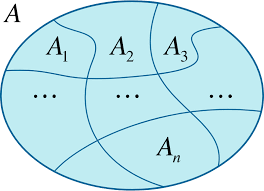
\includegraphics[scale=0.3]{partition.png}
\end{center}
Eine Partition einer Menge A ist eine Menge $\{A_i | i \in I\}$ von
paarweise disjunkten, nichtleeren Teilmengen von A mit
\begin{align*}
    \bigcup_{i \in I} A_i = A
\end{align*}
Die Elemente $A_i$ heissen die Klassen der Partition.werden auch deren Blöcke genannt.
\subsection{Beispiel}
Durch $A_0 = \{2n \mid n \in \mathbb{N}\}$ und $A_1 = \{2n+1 \mid n \in \mathbb{N}\}$ erhält
man eine Partition der natürlichen Zahlen in zwei unendlich grosse Blöcke.

\subsection{Induzierte Partition}
Folgt aus der Reflexivität einer Äquivalenzrelation und der
Äquivalenz:
\begin{align*}
    [a]_{\sim} = [b]_{\sim} \Leftrightarrow [a]_{\sim} \cap [b]_{\sim} \neq \emptyset
\end{align*}
\subsection{Induzierte Äquivalenzrelation}
Ist $P = \{A_i \mid i \in I \}$ eine Partition einer Menge A, dann ist die Relation $\sim$ mit\dots
\begin{align*}
    a \sim b \Leftrightarrow \exists{i} \in I(a \in A_i \wedge b \in A_i)
\end{align*}
...eine Äquivalenzrelation auf A.